\chapter{Background}

\section{Execution Schedule of Spatial Architectures} 
\begin{figure*}
\centering
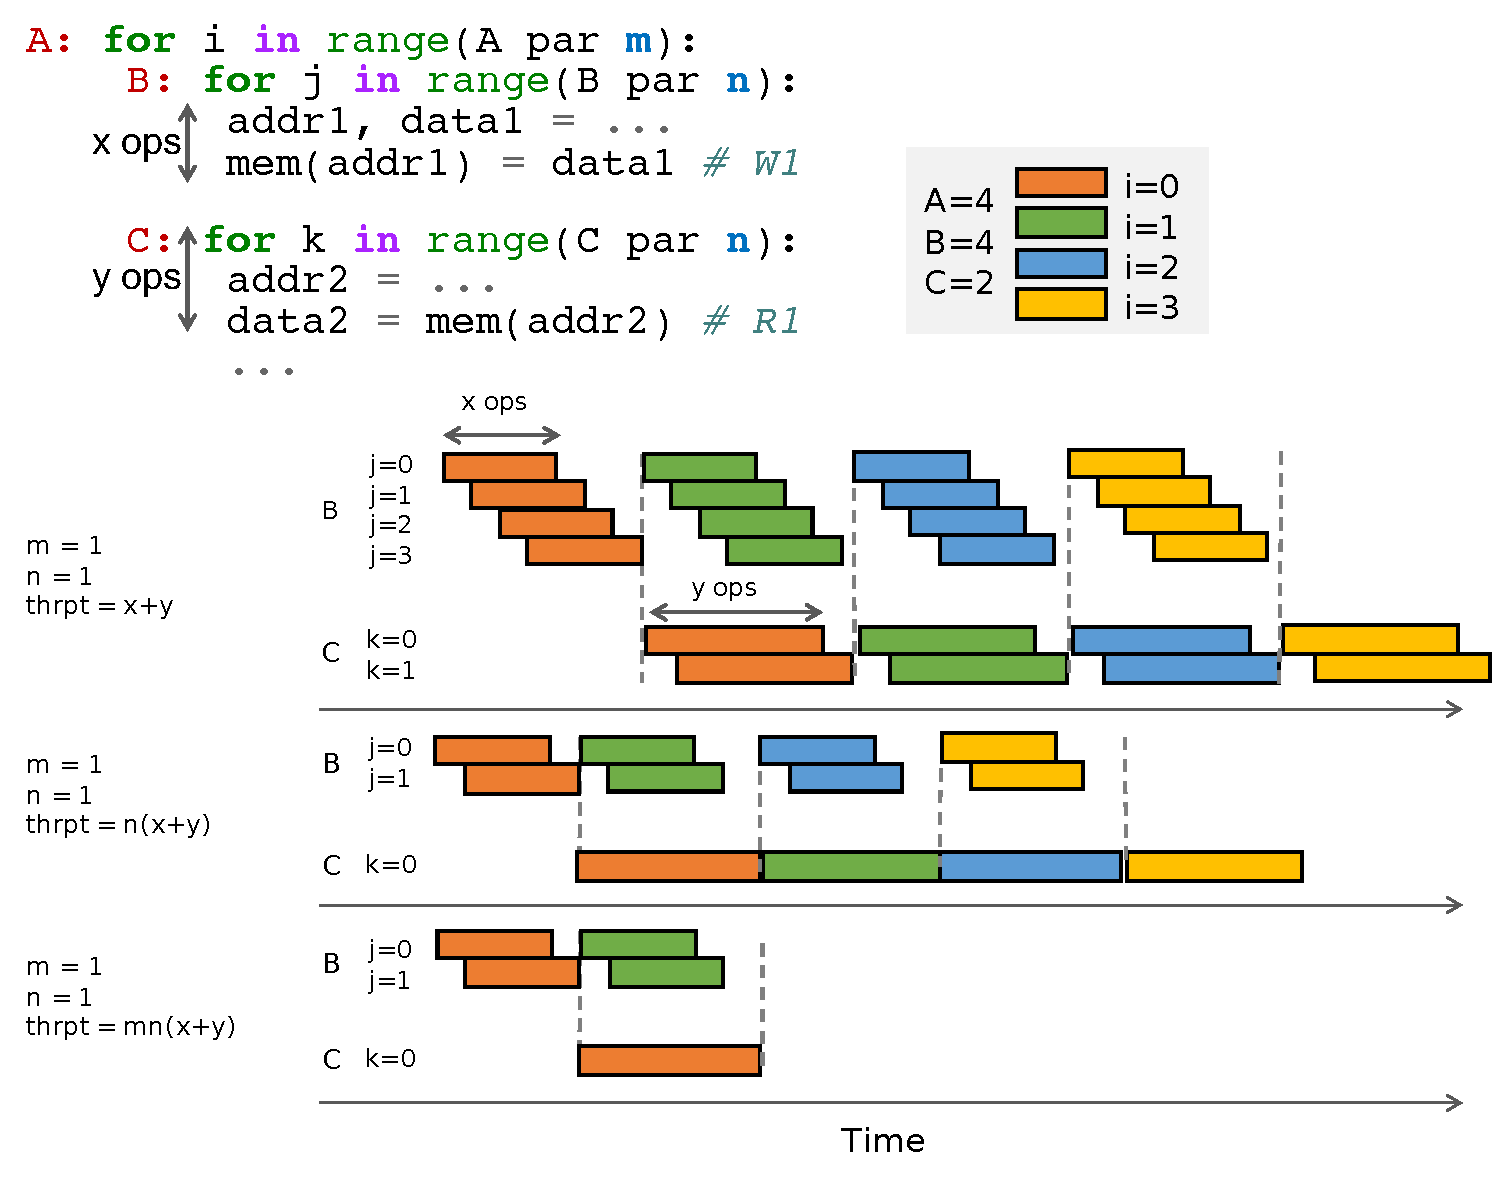
\includegraphics[width=1.0\textwidth]{figs/pipeexec.pdf}
\caption[Hiearchical pipelining and parallelization on spatial architecture]{
Hiearchical pipelining and parallelization in spatial architecture.
(a) illustrates the runtime and throughput of a hiearchically pipelined and parallelized program on
a reconfigurable spatial architecture. 
At inner level, instructions within each basic
block are fine-grained pipelined across iterations of the inner most loop. 
At outer level, the inner loops are coarse-grained pipeliend across the outer loop iterations.
Exploting multiple levels of pipeline parallelism gives a total throughput of $x+y$ operations per cycle.
(b) Vectorizing the inner most loops B and C by \texttt{n} increases the throughput to $(x+y)n$.
(c) Parallelizing the outer loop A by \texttt{m} furhter increases the throughput to $(x+y)mn$.
}
\label{fig:pipeexec}
\end{figure*}

\begin{figure*}
\centering
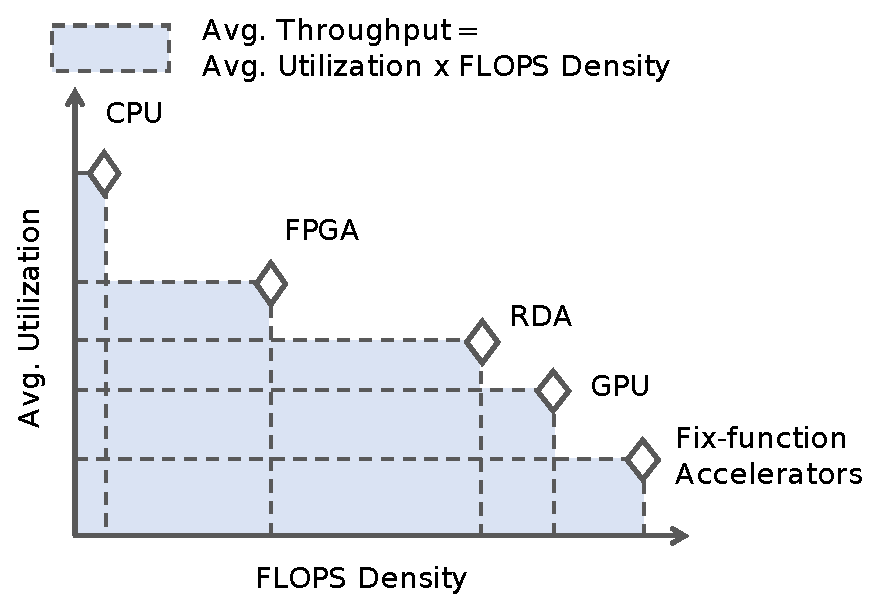
\includegraphics[width=0.6\textwidth]{figs/peakutil.pdf}
\caption[Average utilization vs. peak compute density tradeoff]{
 Average utilization vs. peak compute density tradeoff among different architectures.
}
\label{fig:peakutil}
\end{figure*}

\begin{figure*}
\centering
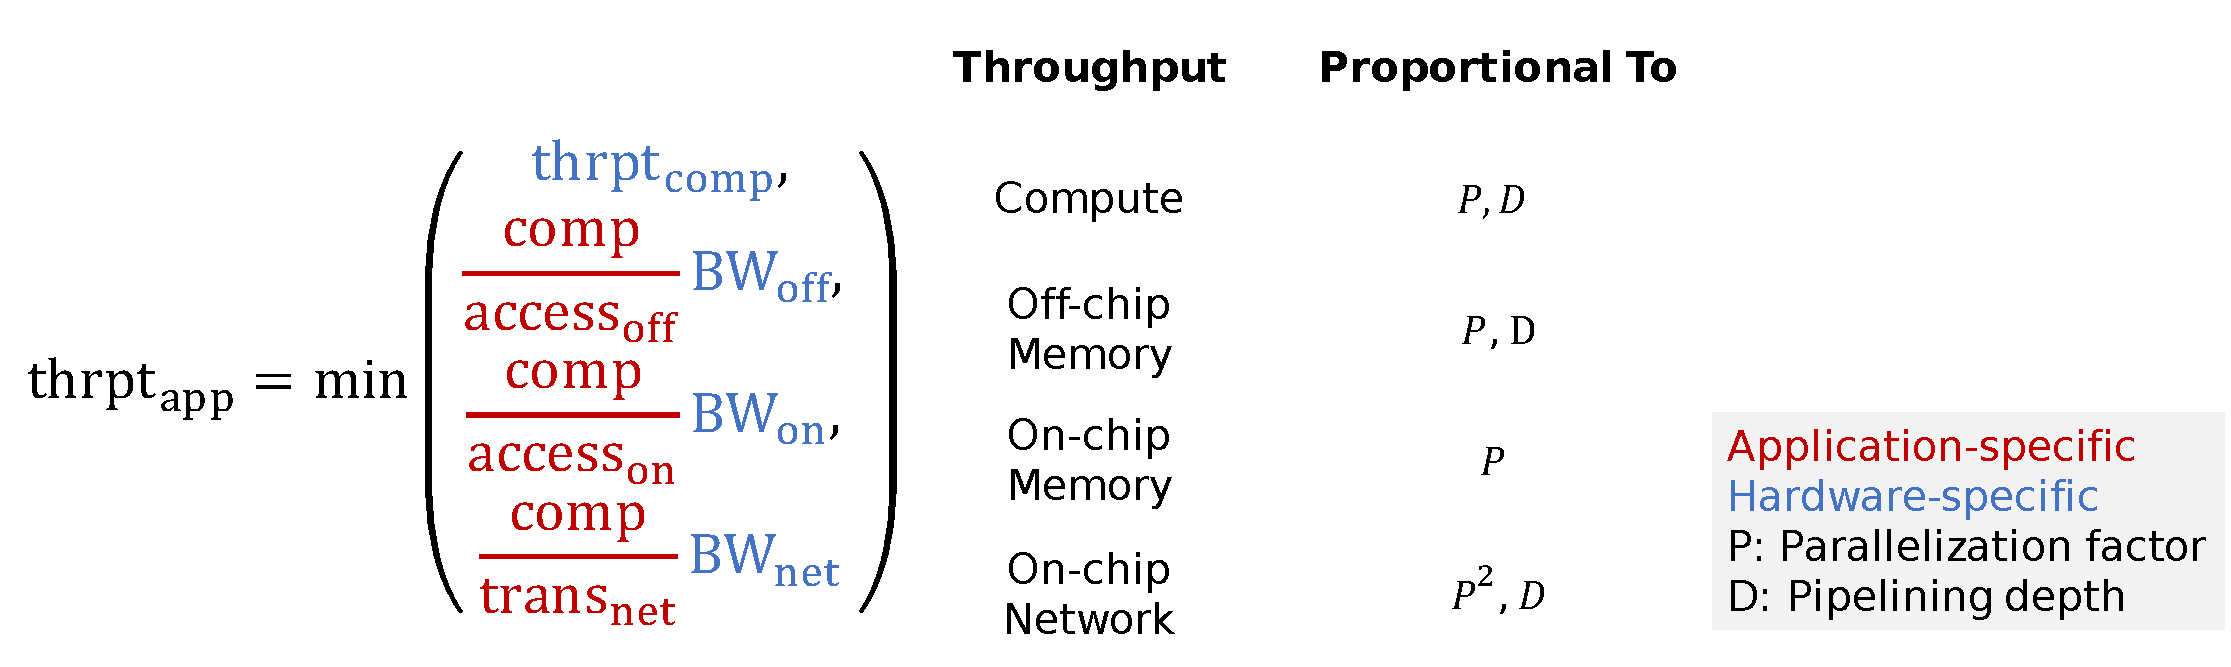
\includegraphics[width=1\textwidth]{figs/perfmodel.pdf}
\caption[High-level performance model of spatial architectures]{
High-level performance model of spatial architectures
}
\label{fig:perfmodel}
\end{figure*}

The biggest advantage of reconfigurable accelerators, compared to processor-based architectures 
such as CPUs and GPUs, is the ability to explore pipeline parallelism at multiple granularity. 

In traditional Von Neumann architectures, a computer consists of a processing unit that performs
computation, a memory unit that stores the program states, and a control unit that tracks execution
states and fetch the instruction to execute. This computing model inheritely assumes that
instructions with in a program are executed in time. 

Unlike traditional Von Neumann architectures, which inheritely assumes program is executed in time, 
reconfigurable data-flow architecutes can statically program 
\gist{pipelined access reduce off-chip access. HBM small capacity}
\gist{scratchpad improves effective bandwidth and capacity}

\Cref{fig:pipeexec} shows an example program executed on the 


\begin{table*}
  \centering
\begin{tabular}{lccc}
  \toprule
 Concurrency Level & Instruction & Data & Task/Kernel  \\ \midrule
 Parallelsim & CPU,\rda & CPU,GPU,\rda & CPU,\rda  \\
 Pipelining & \rda & \rda & \rda \\
 \bottomrule
\end{tabular}
\caption[Concurrency level explored by different architectures]{
  Concurrency level explored by different architectures
}
\label{tab:conclevel}
\end{table*}

\section{Plasticine}

\begin{figure*}
\centering
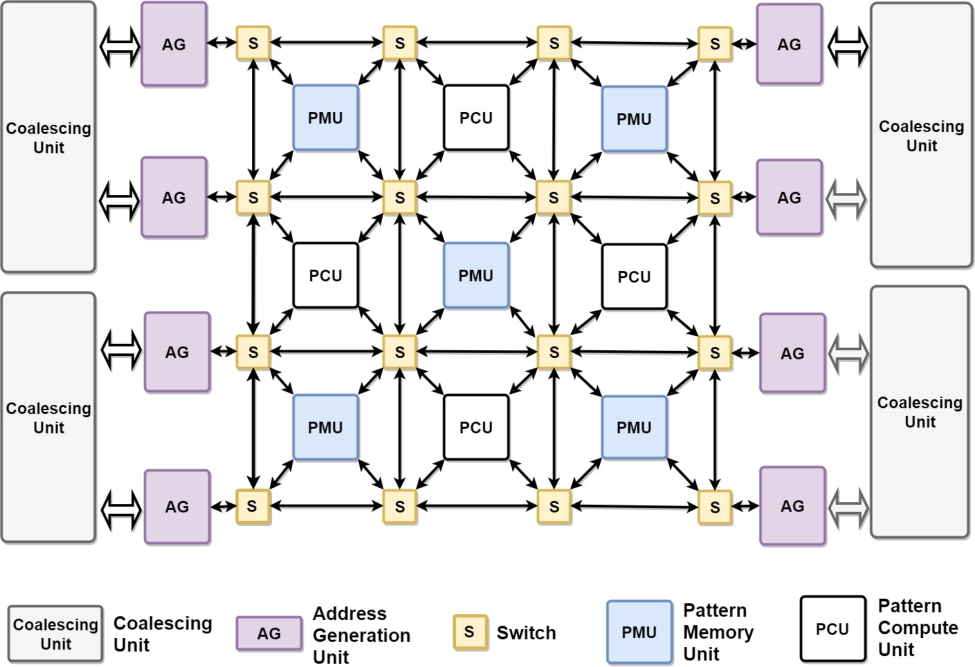
\includegraphics[width=0.8\textwidth]{figs/plasticine.pdf}
\caption[Plasticine chip-level architecture]{Plasticine chip-level architectural diagram}
\label{fig:plasticine}
\end{figure*}

\section{Spatial}

\begin{figure}
\centering
\newsavebox{\outerProduct}
\begin{lrbox}{\outerProduct}
\lstinputlisting[language=Spatial,linewidth=0.91\columnwidth]{code/OuterProduct.scala}
\end{lrbox}
\begin{tabular}{m{0.01cm} l} & \usebox{\outerProduct}\\ \end{tabular}
  %\inputminted[fontsize=\footnotesize]{Scala}{code/OuterProduct.scala}
  \caption{Example of outer product in Spatial pseudocode.}
\label{fig:spatial_app}
\end{figure}

%To target spatial architectures, we use Spatial, an open source domain specific language for reconfigurable accelerators \cite{spatial_koeplinger}.
We use Spatial, an open source domain specific language for reconfigurable accelerators, to target spatial architectures \cite{spatial_koeplinger}.
Spatial describes applications with nested loops and an explicit memory hierarchy that captures data movement on-chip and off-chip. 
This exposes design parameters that are essential for achieving high performance on spatial architectures, including blocking size, loop unrolling factors, inner-loop pipelining, and coarse-grained pipelining of arbitrarily nested loops. 
To enable loop-level parallelization and pipelining, Spatial automatically banks and buffers intermediate memories between loops. 
An example of outer product---element-wise multiplication of two vectors resulting in a matrix---in Spatial is shown in Figure~\ref{fig:spatial_app}.
%In this example we assume inputs \emph{vecA}, \emph{vecB} and outputs \emph{matC} do not fit on chip.
%First, \emph{C2} and \emph{C4} load tiles of vectors of size \emph{tsA} and \emph{tsB} to on-chip scratchpads \emph{tileA} and \emph{tileB}. 
%Next, loop \emph{C5} computes the outer products and store it to scratchpad \emph{tileC}. 
%Finally, \emph{C6} stores partial results back to DRAM. 
\if 0
Spatial enables inner loop pipelining in \emph{C5} and coarse-grained pipelining between stages of the outer loop (e.g. \emph{C4}, \emph{C5}, and \emph{C6} are pipelined across iterations of \emph{C3}). 
The parallelization factor of the inner most loop (\emph{ip} for \emph{C2}, \emph{C5}, and \emph{C6}) translates to SIMD pipeline and vector network vectorization factor. 
In \emph{C1} and \emph{C2}, \emph{op1} and \emph{op2} are outer loop parallelization factors that allow the programmer to unroll the outer loops and parallelize compute, which can better saturates DRAM bandwidth or balances compute pipelines. 
When scratchpad producers or consumers are parallelized, the scratchpad must be banked to sustain the required bandwidth. 
Scratchpads only contain one level of banking hierarchy. 
Therefore, when more than one dimension of the scratchpad is banked, the high-dimensional banks are mapped across multiple scratchpads. 
In this example, if both \emph{ii} and \emph{jj} (used in the write address of \emph{tileC}) on line 31 are parallelized, \emph{tileC} will be mapped to multiple scratchpads. 
This mapping strategy makes broadcast communication common between producers, banks, and consumers when outer loops are unrolled.
\fi
For spatial architectures, Design Space Exploration (DSE) of parameters
(e.g., \emph{op1}, \emph{op2}, \emph{ip}, \emph{tsA}, \emph{tsB}) is critical to achieve good resource utilization and performance \cite{dse_koeplinger}.

